\documentclass[12pt,letterpaper]{article}
% The usepackage tell LaTeX which packages are needed. As you get better you can add more
% packages for extra functionality
% Percent signs are comments, they will not be read by the renderer.
\usepackage{fullpage}
\usepackage[top=2cm, bottom=2.5cm, left=2.5cm, right=2.5cm]{geometry}
\usepackage{amsmath,amsthm,amsfonts,amssymb,amscd}
\usepackage{lastpage}
\usepackage{enumerate}
\usepackage{fancyhdr}
\usepackage{mathrsfs}
\usepackage{xcolor}
\usepackage{graphicx}
\usepackage{multicol}
\usepackage{wrapfig}
\usepackage{hyperref}
\usepackage{systeme}
\usepackage{subfig}
\usepackage[shortlabels]{enumitem}
\usepackage{listings} %for listings of the source code
\usepackage[backend=biber,style=alphabetic,sorting=ynt]{biblatex}

\addbibresource{source2.bib}

% Some definitions for using the listing package.
% When we reference 'codegreen', it will be the RGB color defined below.
\definecolor{codegreen}{rgb}{0,0.6,0}
\definecolor{codegray}{rgb}{0.5,0.5,0.5}
\definecolor{codepurple}{rgb}{0.58,0,0.82}
\definecolor{backcolour}{rgb}{0.95,0.95,0.92}
\DeclareUnicodeCharacter{2212}{-}

% Also for the listings, this will make the code listing look like default MATLAB
\lstdefinestyle{mystyle}{
	backgroundcolor=\color{backcolour},   
	commentstyle=\color{codegreen},
	keywordstyle=\color{magenta},
	numberstyle=\tiny\color{codegray},
	stringstyle=\color{codepurple},
	basicstyle=\footnotesize,
	breakatwhitespace=false,         
	breaklines=true,                 
	captionpos=b,                    
	keepspaces=true,                 
	numbers=left,                    
	numbersep=5pt,                  
	showspaces=false,                
	showstringspaces=false,
	showtabs=false,                  
	tabsize=2
}
\lstset{style=mystyle}

\hypersetup{%
  colorlinks=true,
  linkcolor=blue,
  linkbordercolor={0 0 1}
}

 
\setlength{\parindent}{0.0in}
\setlength{\parskip}{0.05in}

\newcommand\course{COMP 521}          
\newcommand\MyName{Zachary Humphries}  

\pagestyle{fancyplain}
\headheight 15pt
\lhead{\MyName}
%\lhead{\NetIDa\\\NetIDb}                 % <-- Comment this line out for problem sets (make sure you are person #1)
\chead{\textbf{\Large Final Project Report}}
\rhead{\course\\ December 15, 2022}
\lfoot{}
\cfoot{}
\rfoot{\small\thepage}
\headsep 1.5em

\begin{document}

\section*{Background}
The Black-Scholes Model is a partial differential equation (PDE) developed by Fisher Black and Myron Scholes to evaluate the underlying price of European options. 
An option is an agreement where someone can reserve to buy (call) or sell (put) a stock at specific time. 
Unlike American options, European options can only be exercised at the maturity date.
\vspace*{0.10in}

I chose to work on this PDE because I had experience with the equation while working as a pricing analyst in the natural gas industry, but never really understood the equation.
The Risk Management team that worked alongside the Pricing team would mitigate risk (hedge) by buying call options on future consumption of natural gas by customers, whose contracts we would price.
\vspace*{0.10in}

The research paper \textit{\textbf{Examination of Impact from Different Boundary Conditions on the 2D Black-Scholes Model:} Evaluating Pricing of European Call Options} by Tomas Sundvall and David Trång\cite{sundvall-trang-2014} informed this project.

\vspace*{0.10in}

\section*{Black-Scholes Model}
The Black-Scholes model is defined by the partial differencial equation\ldots

\begin{equation*}
    F_{t} = -rxF_{x}-ryF_{y}-\frac{1}{2}x^{2}\sigma^{2}(1,1)F_{xx} -\frac{1}{2}y^{2}\sigma^{2}(2,2)F_{yy}-xy\sigma^{2}(1,2)F_{xy}+rF
\end{equation*}

With $x$ and $y$ representing the hypothetical price of two assets with some volatility correlationship to each other.

The payoff function at the maturity time is:

\begin{equation*}
    F(T,x,y) = \Phi(x,y) = \left(\frac{x+y}{2}-K\right)^{+}
\end{equation*}

The parameters in the equation are:
\begin{itemize}
    \item $r:$ Risk-free Investment (often US bonds)
    \item $\sigma:$ Volitility Correlation Matrix \begin{equation*}\sigma = \begin{pmatrix}
        \sigma_{xx}  & \sigma_{yx}  \\
        \sigma_{xy}  & \sigma_{yy}
    \end{pmatrix},\hspace{0.5cm} \sigma_{yx} = \sigma_{xy},\hspace{0.5cm} \sigma_{xx} = \sigma_{yy}\end{equation*}
    \item $T:$ Final Maturity Time
    \item $K:$ Strike Price (Call Option Premium)
\end{itemize}

\newpage
\section*{Parameters}

As used in the paper by Sundvall and Trångor the project, I will be using the parameters:
\begin{itemize}
    \item $r=0.1$
    \item $\sigma(1,1) = 0.3$
    \item $\sigma(1,2) = 0.05$
\end{itemize}

Being undefined in the paper, I will also be using the parameters:
\begin{itemize}
    \item $T=1$
    \item $K=1$
\end{itemize}

The following code displays the implementation of the parameters

\lstset{title={Initial Values}}
\begin{lstlisting}[language = Matlab]
%% Parameters

strike = 1;                 % Strike Price
T = 1;                      % Simulation time or Final Maturity Time

a = 0;                      % Minimum Value of Option for Asset X (must be zero)
b = round(10*strike);       % Maximum Value of Option for Asset X per recommendation of reference paper (between 8*K and 12*K)
c = 0;                      % Minimum Value of Option for Asset Y (must be zero)
d = b;                      % Maximum Value of Option for Asset X

m = 8* round(10*strike);    % Personal Preference: Gives Enough Divisions for a More Accurate Result
n = m;                      % Number of cells along the y-axis

dx = (b-a)/m;               % Step length along the x-axis
dy = (d-c)/n;               % Step length along the y-axis


dt = 0.001;                 % Personal Preference: Much less than Von Neumann stability criterion for explicit scheme dx^2/(4) (about 0.0039)

omega11 = 0.3;              % Omega_xx = Omega_yy of the volatility correlation matrix
omega12 = 0.05;             % Omega_xy = Omega_yx of the volatility correlation matrix
r = 0.1;                    % Risk free interest rate
\end{lstlisting}

\newpage

\section*{Initial Values}
Since the value of the option is discounted to the present, the initial condition is the payoff function:

\begin{equation*}
    F(T,x,y) = \Phi(x,y) = \left(\frac{x+y}{2}-K\right)^{+}
\end{equation*}

This initial value is displayed in the code below:

\lstset{title={Initial Values}}
\begin{lstlisting}[language = Matlab]
%% Initial Values for time = T

ICV = max(((X+Y)/2)-strike, 0);
\end{lstlisting}


\newpage

\section*{Dirichlet Boundary Conditions}
By the nature of options having a minimum value of zero (lower domain) but no maximum price, the boundary conditions are divided into close-field and far-field boundary conditions.


Shown below, are the close-field (as diamonds) and far-field (as stars) boundary conditions. The triangular points where the close-field boundary conditions and meet the far-field boundary conditions can be either of the two, however, in this project, they are defined as far-field boundary conditions.
The far-field boundary condition will be updated with each time step with the close-field boundary conditions being encorporated into the inverted matrix, $A$.
\\

\begin{figure}[!h]
    \centering
    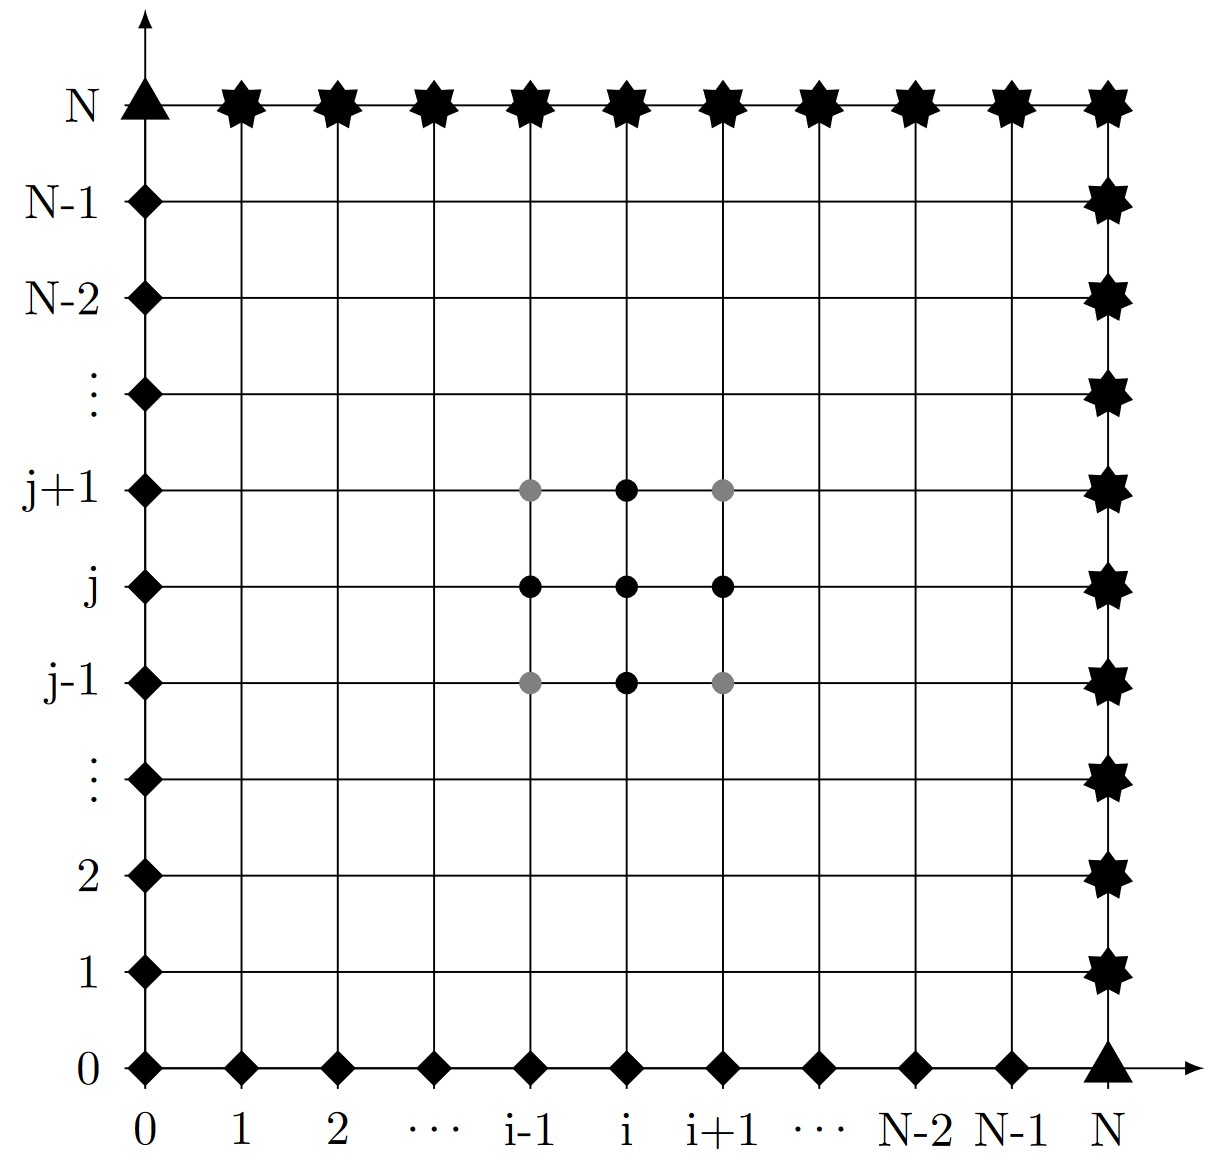
\includegraphics[width=.8\linewidth]{boundary-graph.jpg}\label{fig:Boundary Conditions Graph}
\end{figure}

\newpage
\subsection*{Close-Field Boundary Conditions}

Due to $y=0$ on the x-axis and $x=0$ on the y-axis, the x and y axes simplify as:

\begin{equation*}
\begin{matrix}
    F_{t} = -rxF_{x}-\frac{1}{2}x^{2}\sigma^{2}(1,1)F_{xx}+rF \\
    \\
    F_{t} = -ryF_{y}-\frac{1}{2}y^{2}\sigma^{2}(2,2)F_{yy}+rF
\end{matrix}
\end{equation*}

The value at the origin $F(t,0,0) = 0$.


\subsection*{Far-Field Boundary Conditions}
Extrapolating the 1D case of the limit as the payoff function goes to infinity into 2D, the paper defined the far-field boundary conditions as:

\begin{equation*}
\begin{matrix}
    F(t,x_{max},y) = \frac{x_{\text{max}}+y}{2}-Ke^{-r(T-t)}\\
    \\
    F(t,x,y_{max}) = \frac{x+y_{\text{max}}}{2}-Ke^{-r(T-t)}
\end{matrix}
\end{equation*}

The paper notes, as a "rule of thumb”, to limit the upper domain by setting the $x_{\text{max}}$ and $y_{\text{max}}$ to 4K to 6K times the number of spatial dimensions (two in this case).
In this case, I have decided to use 10K as the upper limit for both x and y.

\newpage

\section*{Discretization in Space}

Following the same method as the refered paper, this section will cover the derivative matricies using central differences of second order accuracy:

\begin{equation*}
\begin{matrix}
\begin{matrix}
    \left(\frac{\partial F}{\partial x}\right)_{i,j} \approx \frac{U_{i+1,j}-U_{i-1,j}}{2\Delta x}, & \left(\frac{\partial^2 F}{\partial x^2}\right)_{i,j} \approx \frac{U_{i+1,j}+2U_{i,j}+U_{i-1,j}}{\Delta x^2},\\
    \\
    \left(\frac{\partial F}{\partial y}\right)_{i,j} \approx \frac{U_{i,j+1}-U_{i,j-1}}{2\Delta y}, & \left(\frac{\partial^2 F}{\partial y^2}\right)_{i,j} \approx \frac{U_{i,j+1}+2U_{i,j}+U_{i,j-1}}{\Delta y^2},\\
\end{matrix} 
    \\
    \\
    \left(\frac{\partial^2 F}{\partial x \partial y}\right)_{i,j} \approx \frac{U_{i+1,j+1}-U_{i+1,j-1}-U_{i-1,j+1}+U_{i-1,j-1}}{4\Delta x \Delta y}
\end{matrix}
\end{equation*}

The Black-Scholes equation can be reconstructed with these approximations as\ldots

\begin{equation*}
    \begin{aligned}
        \left(\frac{\partial F}{\partial t}\right)_{i,j} \approx & -rx \frac{U_{i+1,j}-U_{i-1,j}}{2\Delta x} -ry \frac{U_{i+1,j}+2U_{i,j}+U_{i-1,j}}{\Delta x^2}\\
        & - \frac{\sigma^{2}(1,1)x^2}{2}\frac{U_{i+1,j}+2U_{i,j}+U_{i-1,j}}{\Delta x^2} - \frac{\sigma^{2}(2,2)y^2}{2}\frac{U_{i,j+1}+2U_{i,j}+U_{i,j-1}}{\Delta y^2}\\
        & - \sigma^{2}(1,2)xy \frac{U_{i+1,j+1}-U_{i+1,j-1}-U_{i-1,j+1}+U_{i-1,j-1}}{4\Delta x \Delta y} + r U_{i,j}
    \end{aligned}
\end{equation*}

One point to notes is that since the goal is to create an implicit euler scheme, in order to make the invertable matrix, $A$, I will be making $\left(\frac{\partial}{\partial t}\right)_{i,j}$ and later applying $F$.

\subsection*{Implementing $A = \left(\frac{\partial}{\partial t}\right)_{i,j}$ Not Including Boundary Conditions}
The MATLAB code below displays the implementation of $A = \left(\frac{\partial}{\partial t}\right)_{i,j}$. All rows corresponding to the near and far boundary conditions are left blank in this process.

\lstset{title={Implementation of $\left(\frac{\partial}{\partial t}\right)_{i,j}$}}
\begin{lstlisting}[language = Matlab]
%% Setting Up Matrix for Fx

Fx = Fx_Matrix(m,n,dx,dy);                          % 2nd Order 2D Scheme for First Derivative with Respect to X
Fy = Fy_Matrix(m,n,dx,dy);                          % 2nd Order 2D Scheme for First Derivative with Respect to Y

Fxx = Fxx_Matrix(m,n,dx,dy);                        % 2nd Order 2D Scheme for Second Derivative with Respect to X
Fyy = Fyy_Matrix(m,n,dx,dy);                        % 2nd Order 2D Scheme for Second Derivative with Respect to Y

Fxy = Fxy_Matrix(m,n,dx,dy);                        % 2nd Order 2D Scheme for Mixed Derivative with Respect to X and Y

sub_matrix = diag(diag(comp_matrix("x", m, n)));    % Matrix to Subtract from speye so All Boundary Conditions in A are Zero

%% Using Black-Scholes PDE to Create A (Excluding Boundary Conditions)

A = (-r*Xmatrix*Fx) - (r*Ymatrix*Fy) - ((1/2)*omega11^2*Xmatrix*Xmatrix * Fxx) - ((1/2)*omega11^2*Ymatrix*Ymatrix * Fyy) - (omega12^2*Xmatrix*Ymatrix*Fxy) + (r*(speye((m+1)*(n+1))-sub_matrix));
\end{lstlisting}


\lstset{title={Functions for $\left(\frac{\partial}{\partial t}\right)_{i,j}$}}
\begin{lstlisting}[language = Matlab]
    function matrixdx = Fx_Matrix(m,n,dx,dy)
    one = ones(m+1,1);
    sparse_m = sparse(m+1,1);
    A = spdiags([-1*one sparse_m one],-1:1,m+1,m+1);
    A(1,:) = sparse_m';
    A(end,:) = sparse_m';

    sparse_y = speye(n+1,n+1);
    sparse_n = sparse(n+1,1);
    sparse_y(:,1) = sparse_n;
    sparse_y(:,end) = sparse_n;
 
    matrixdx = kron(sparse_y, A)/(2*dx);
end

function matrixdy = Fy_Matrix(m,n,dx,dy)
    one = ones(n-1,1);
    sparse_n = sparse(n+1,1);
    one = sparse([0;one;0]);
    one_list = repmat(one,m-1,1);
    one_list1 = [sparse_n; one_list; sparse_n];
    one_list2 = [sparse_n; one_list; sparse_n];

    A = spdiags([-1*one_list1 repmat(sparse_n, n+1, 2*(m+1)-1) one_list2],-(m+1):(m+1),(m+1)*(n+1),(m+1)*(n+1));
 
    matrixdy = -1*(((A)/(2*dy))');
end

function matrixdxx = Fxx_Matrix(m,n,dx,dy)
    one = ones(m+1,1);
    sparse_m = sparse(m+1,1);
    A = spdiags([one -2*one one],-1:1,m+1,m+1);
    A(1,:) = sparse_m';
    A(end,:) = sparse_m';

    sparse_y = speye(n+1,n+1);
    sparse_n = sparse(n+1,1);
    sparse_y(:,1) = sparse_n;
    sparse_y(:,end) = sparse_n;
 
    matrixdxx = kron(sparse_y, A)/(dx^2);
end

function matrixdyy = Fyy_Matrix(m,n,dx,dy)
    one = ones(n-1,1);
    sparse_n = sparse(n+1,1);
    one = sparse([0;one;0]);
    one_list = repmat(one,m-1,1);
    one_list1 = [sparse_n; one_list; sparse_n];
    one_list2 = [sparse_n; one_list; sparse_n];
    diag = [sparse_n; one_list; sparse_n];
    
    A = spdiags([one_list1 repmat(sparse_n, n+1, m) -2*diag repmat(sparse_n, n+1, m) one_list2],-(m+1):(m+1),(m+1)*(n+1),(m+1)*(n+1));
 
    matrixdyy = ((A)/(dy^2))';
end

function matrixdxy = Fxy_Matrix(m,n,dx,dy)
    one = ones(n-1,1);
    sparse_n = sparse(n+1,1);
    one1 = sparse([0;one;0]);
    one2 = sparse([0;one;0]);
    one_list = repmat(one1,m-1,1);
    one_list2 = repmat(one2,m-1,1);
    one_list1 = [sparse_n; one_list; sparse_n];
    one_list2 = [sparse_n; one_list2; sparse_n];
    one_list3 = [sparse_n; one_list2; sparse_n];
    one_list4 = [sparse_n; one_list; sparse_n];

    sparse_list = repmat(sparse_n,m+1,1);

    diags1 = [one_list1 sparse_list -1*one_list2];

    diags2 = [one_list1 sparse_list -1*one_list2];


    A1 = spdiags(diags1,-(m+1)-1:-(m+1)+1,(m+1)*(n+1),(m+1)*(n+1));

    A2 = spdiags(diags2,(m+1)-1:(m+1)+1,(m+1)*(n+1),(m+1)*(n+1));

    A = A1+A2;

    matrixdxy = ((A)/(4*dy*dy))';
end

function A = comp_matrix(yee, m, n)
    bc_matrix = sparse(m+1,n+1);
    bc_matrix(1,:) = 1;
    bc_matrix(end,:) = 1;
    bc_matrix(:,1) = 1;
    bc_matrix(:,end) = 1;
    
    bc_list = reshape(bc_matrix, (m+1)*(n+1),1);
    bc_matrix = repmat(bc_list, 1, (m+1)*(n+1));

    if yee=="x"
        A = bc_matrix;
    else
        A = bc_matrix';
    end
end
\end{lstlisting}

\subsection*{Including Close-Field Boundary Conditions into $A = \left(\frac{\partial}{\partial t}\right)_{i,j}$}

As mentioned previously, the equations dictating the boundary conditions on the x-axis and y-axis, in order, are\ldots

\begin{equation*}
\begin{matrix}
    F_{t} = -rxF_{x}-\frac{1}{2}x^{2}\sigma^{2}(1,1)F_{xx}+rF \\
    \\
    F_{t} = -ryF_{y}-\frac{1}{2}y^{2}\sigma^{2}(2,2)F_{yy}+rF
\end{matrix}
\end{equation*}

The MATLAB code below displays the encorporation of the close-field boundary conditions\ldots

\lstset{title={Encorporation of the Close-Field Boundary Conditions}}
\begin{lstlisting}[language = Matlab]
%% Encorporating Close-Field Boundary Conditions into A

Fx_1D = Derivative_1D_Matrix(m,dx);                 % 2nd Order 1D Scheme for First Derivative with Respect to X
Fy_1D = Derivative_1D_Matrix(n,dy);                 % 2nd Order 1D Scheme for First Derivative with Respect to Y
Fxx_1D = Double_Derivative_1D_Matrix(m,dx);         % 2nd Order 1D Scheme for Second Derivative with Respect to X
Fyy_1D = Double_Derivative_1D_Matrix(n,dy);         % 2nd Order 1D Scheme for Second Derivative with Respect to Y

Xmatrix_1D = diag(xgrid');
Ymatrix_1D = diag(ygrid');

I_1D = speye(m+1,n+1);                              % Origin and Far-Field Boundary Conditions Are Later Addressed
I_1D(end,end) = 0;
I_1D(1,1) = 0;

xaxis = ((-r * Xmatrix_1D*Fx_1D) - (1/2 * omega11^2 * Xmatrix_1D*Xmatrix_1D * Fxx_1D) + r*I_1D);
yaxis = ((-r * Ymatrix_1D*Fy_1D) - (1/2 * omega11^2 * Ymatrix_1D*Ymatrix_1D * Fyy_1D) + r*I_1D);


A(1:m+1, 1:n+1) = sparse(xaxis);                    % Inserting Close-Field Boundary Condition for X-Axis into A

row_insert = [1:m+1:(m+1)*(n+1)];                   % Resizing Y to be Inserted Into A Matrix
yaxis_matrix1 = sparse((m+1)*(n+1),m+1);
yaxis_matrix1(row_insert,:) = yaxis;
col_insert = [1:n+1:(n+1)*(m+1)];
yaxis_matrix2 = sparse((m+1)*(n+1),(m+1)*(n+1));
yaxis_matrix2(:, col_insert) = yaxis_matrix1;

A = A+yaxis_matrix2;                                % Inserting Close-Field Boundary Condition for Y-Axis into A
\end{lstlisting}

\lstset{title={Functions Used for Encorporation of the Close-Field Boundary Conditions}}
\begin{lstlisting}[language = Matlab]
function matrixdx = Derivative_1D_Matrix(m,dx)
    one = ones(m+1,1);
    sparse_m = sparse(m+1,1);
    A = spdiags([-1*one sparse_m one],-1:1,m+1,m+1);
    A(1,:) = sparse_m';
    A(end,:) = sparse_m';
 
    matrixdx = (A)/(2*dx);
end

function matrixdxx = Double_Derivative_1D_Matrix(m,dx)
    one = ones(m+1,1);
    sparse_m = sparse(m+1,1);
    A = spdiags([one -2*one one],-1:1,m+1,m+1);
    A(1,:) = sparse_m';
    A(end,:) = sparse_m';

    matrixdxx = (A)/(dx^2);
end
\end{lstlisting}

\subsection*{Adjusting $A = \left(\frac{\partial}{\partial t}\right)_{i,j}$ to Account for Far-Field Boundary Conditions}

As the value of the far-field boundary conditions are predefined, ones will be inserted into the diagonals of the A matrix corresponding to the positions of the far-field boundary.

The following MATLAB code shows such implementation\ldots

\lstset{title={Updating $A$ for Far-Field Boundary Conditions}}
\begin{lstlisting}[language = Matlab]
%% Updating A to Account for Far-Field Dirichlet Boundary Conditions

dirichlet_far = zeros((m+1),(n+1));
dirichlet_far(end,:) = ones(length(xgrid),1);
dirichlet_far(:,end) = ones(length(ygrid),1);

dirichlet_far = diag(reshape(dirichlet_far, 1, (m+1)*(n+1)));

A = sparse(A+dirichlet_far);                    % Values Corresponding to Far-Field Boundary in A Are One on Diagonal
A(1,1) = 1;                                     % Origin is Always Zero
\end{lstlisting}

\newpage

\section*{Discretization in Time}

Given that the Black-Scholes model approximates the first derivative with respect to time ($F_t$), the true payoff function $F$ will need to be approximated through time as well.

Rewriting in the form of ($Ax+b$), where $A$ is the contructed matrix approximating $\left(\frac{\partial}{\partial t}\right)_{i,j}^n$ including boundary conditions, $U^n$ is a vector the value of the $F$ at time, $n$, and $b^n$ is a vector of the dirichlet boundary values at time $n$, gives\ldots

\begin{equation*}
    \left(\frac{\partial U}{\partial t}\right)^n = AU^n - b^n
\end{equation*}

\subsection*{Second-Order Implicit Euler Scheme}
Since the value is discounted back to the present, the equation above can be rewritten in terms of $U^{n-1}$ as\ldots

\begin{equation*}
    \begin{aligned}
    \left(\frac{\partial U}{\partial t}\right)^{n-1} \approx \frac{U^{n}-U^{n-1}}{\Delta t} + \frac{\Delta t}{2}\frac{U^{n-1}-2U^{n}+U^{n+1}}{\Delta t^2} = AU^{n-1} - b^{n-1}
    \end{aligned}
\end{equation*}

Solving for $U^{n-1}$\ldots

\begin{equation*}
    \frac{U^{n}}{\Delta t} + \frac{\Delta t}{2}\frac{U^{n-1}-2U^{n}+U^{n+1}}{\Delta t^2} + b^{n-1} = AU^{n-1} + \frac{U^{n-1}}{\Delta t} - \frac{U^{n-1}}{2\Delta t} 
\end{equation*}

\begin{equation*}
    \frac{U^{n}}{\Delta t} + \frac{\Delta t}{2}\frac{U^{n-1}-2U^{n}+U^{n+1}}{\Delta t^2} + b^{n-1} = \left(A + \frac{1}{2\Delta t}\right)(U^{n-1})
\end{equation*}

\begin{equation*}
    U^{n-1} = \left(A + \frac{1}{2\Delta t}\right)^{-1} \left(\frac{U^{n}}{\Delta t} + \frac{\Delta t}{2}\frac{U^{n-1}-2U^{n}+U^{n+1}}{\Delta t^2} + b^{n-1}\right)
\end{equation*}

However, because the first time-step is not defined, it will be approximated by the first-order implicit scheme\ldots

\begin{equation*}
    \frac{U^{n}-U^{n-1}}{\Delta t} = AU^{n-1} - b^{n-1}
\end{equation*}
\begin{equation*}
    U^{n-1} = \left(A + \frac{1}{\Delta t}\right)^{-1} \left(\frac{U^{n}}{\Delta t} + b^{n-1}\right)
\end{equation*}

This will result in the scheme being only first-order accurate, which will be analyzed in later sections.

The following code shows the implementation of the time discretization\ldots

\lstset{title={Time Discretization}}
\begin{lstlisting}[language = Matlab]
%% 1st Order Time Scheme to Calculate U After First Time Step

U = reshape(ICV, (m+1)*(n+1), 1);

U_minus = U;
BC_minus = BC;

U = inv((speye(size(A))+(dt*A)))*U_minus+(dt*BC_minus);

U = U-BC;

BC = reshape(BC,(m+1),(n+1));
upperx = ((xgrid+d)/2)-(strike*exp(-r*(T)));    % Updating Far-Field Boundary Conditions for X
uppery = ((b+ygrid)/2)-(strike*exp(-r*(T)));    % Updating Far-Field Boundary Conditions for Y

BC(end,:) = upperx;
BC(:,end) = uppery;
BC = reshape(BC,(m+1)*(n+1), 1);

U = reshape(U,(m+1),(n+1));
U(end,:) = 0;
U(:,end) = 0;
U = reshape(U,(m+1)*(n+1), 1);

U = U + BC;                                     % Making Sure Far-Field Boundaries Have Correct Value in Case of Rounding Error

%% Calculate Inverse of Matrix Needed for 2nd Order Implicit Time Scheme

A_second_order = inv(A+((1/(2*dt))*speye(size(A))));

%% Time Integration Loop
% Note: Value is Being Discounted back to the Present from Exersize Date

count = 1;
len = length(dt : dt : T)-1;

for t = dt : dt : T-dt 
    fprintf("%f ",count)
    fprintf("%f \n",len)

    count = count + 1;

    top = ((((U-BC))/dt)+((dt/2)*((-2*(U-BC) + (U_minus-BC_minus))/(dt*dt))) + BC); % Updating Implicit Scheme Vector

    top = reshape(top,(m+1),(n+1));                 % Making Sure Far-Field Boundaries Have Correct Value in Case of Rounding Error
    top(end,:) = 0;
    top(:,end) = 0;
    top = reshape(top,(m+1)*(n+1), 1);
    top = top + BC;

    U_plus = A_second_order*top;                    % 2nd Order Implicit Scheme for Next Time Step

    BC_minus = BC;

    BC = reshape(BC,(m+1),(n+1));
    upperx = ((xgrid+d)/2)-(strike*exp(-r*(T-t)));  % Updating Far-Field Boundary Conditions for X
    uppery = ((b+ygrid)/2)-(strike*exp(-r*(T-t)));  % Updating Far-Field Boundary Conditions for Y

    BC(end,:) = upperx;
    BC(:,end) = uppery;
    BC = reshape(BC,(m+1)*(n+1), 1);

    U_plus = reshape(U_plus,(m+1),(n+1));
    U_plus(end,:) = 0;
    U_plus(:,end) = 0;
    U_plus = reshape(U_plus,(m+1)*(n+1), 1);
    
    U_plus = U_plus + BC;

    U_minus = U;                                    % Updating U_minus and U for Next Time Step
    U = U_plus;

end
\end{lstlisting}


\newpage

\section*{Results}

As done in the refered paper, this section will focus on the area encompassing $\left[0\leq x \leq \frac{5K}{3}\right]$ and $\left[0\leq y \leq \frac{5K}{3}\right]$ for the approximated F at time, $t=0$.

\begin{figure}[!h]
    \centering
    \subfloat{
    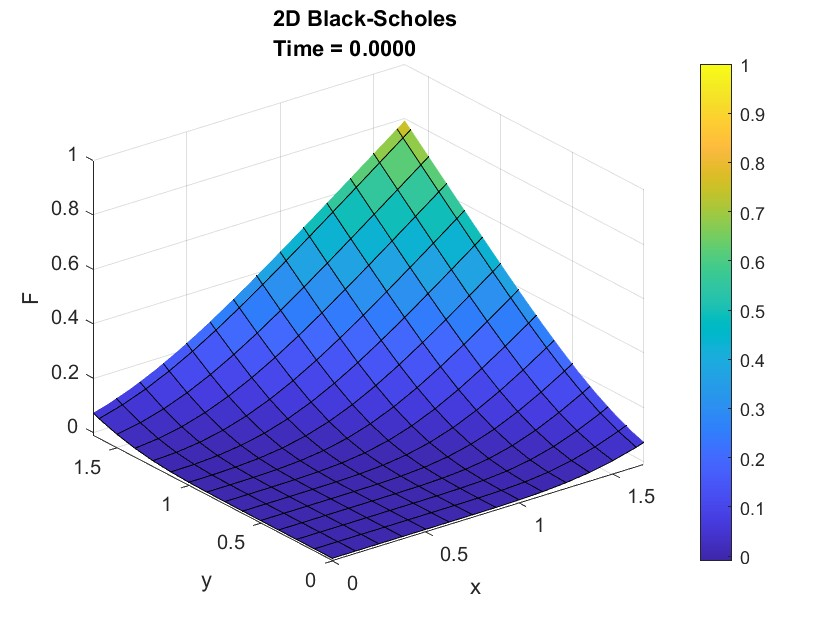
\includegraphics[width=.5\textwidth]{result.jpg}
    }
    \subfloat{
    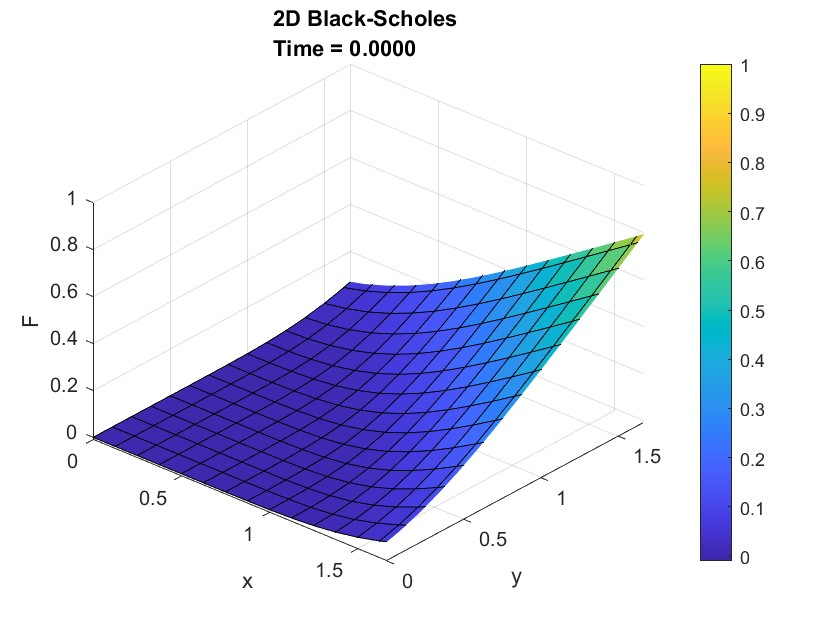
\includegraphics[width=.5\textwidth]{result_2.jpg}
    }
    
    \caption{Approximated $F$ around $\left[0\leq x \leq \frac{5K}{3}\right]$ and $\left[0\leq y \leq \frac{5K}{3}\right]$}
\end{figure}

The figures show a curve similar to the 1D case of the Black-Scholes model, however extrapolated to two dimensions.

\section*{Error Analysis}

For the error analysis, based off of the initial $\Delta t = 10^{-3} = 0.001$,  I chose the differing $\Delta t$ list as\ldots

\begin{equation*}
    \Delta t = \left[\frac{10^{-3}}{2}, \frac{10^{-3}}{4}, \frac{10^{-3}}{8}, \frac{10^{-3}}{16}, \frac{10^{-3}}{32}\right] 
\end{equation*}

I chose the time step $\Delta t = \frac{10^{-3}}{64}$ as the most accurate time-step of comparison because the order of accuracy between the time step $\Delta t = \frac{10^{-3}}{32}$ and $\Delta t = \frac{10^{-3}}{64}$ (shown below) was not majorly affected. 
I also chose the point, $F_{x=1.25, y=1.25}$, instead of the midpoint because since maximum value of $x$ and $y$ can technically be infinite, a value near the strike price, $K=1$, would be more relevant.

The following log-log plot displays the order of accuracy for the system\ldots

\newpage

\begin{figure}[!h]
    \centering
    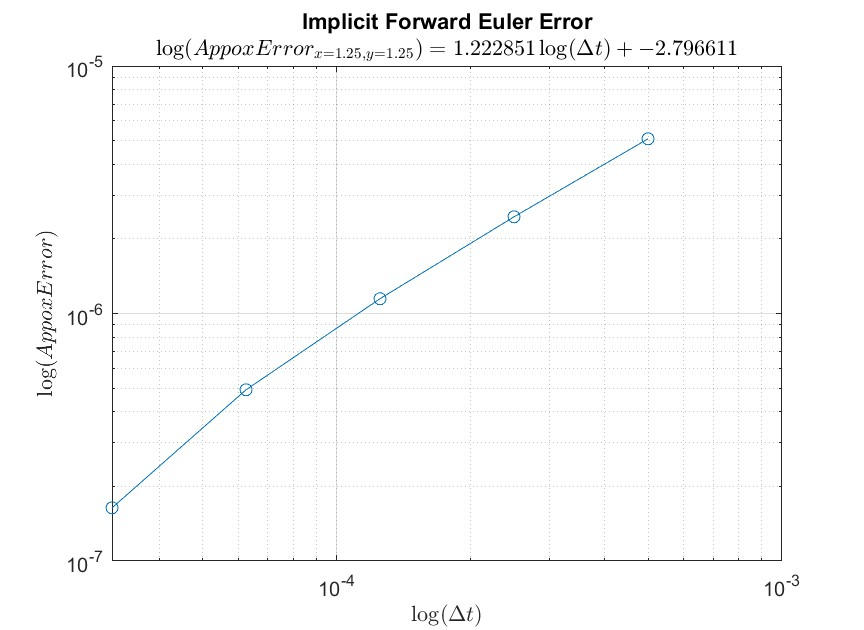
\includegraphics[width=1\linewidth]{error_plot.jpg}\label{fig:Error Plot}
\end{figure}

Even though the time discretization was second-order accurate, with the estimation of the initial $U^{n}$ being only first-order accurate, the first-order accuracy \"flowed\" into the system, leaving it only first-order accurate ($\approx 1.22$).

\section*{Personal Reflection}

In the future, I would update the system to be second-order accurate by creating a \"ghost\" time-step before the time, $t=T$. Due to time constraints and this problem being already rather complex, I did not implement this idea.

I greatly appreciate Jared Brzenski for his guidance for this Black-Scholes model project, as well as his insights for my COMP-670 project for the same model using mimetic operators.

\newpage

\printbibliography

\newpage

\section*{Appendix: MATLAB Code}

\lstset{title={COMP\_521\_Final\_Project\_Black\_Scholes\_Zachary\_Humphries\.m}}
\begin{lstlisting}[language = Matlab]
%% 2D Black-Scholes PDE
% Zachary Humphries
% COMP 521
% Fall 2022

clear
close all

%% Parameters

strike = 1;                 % Strike Price
T = 1;                      % Simulation time or Final Maturity Time

a = 0;                      % Minimum Value of Option for Asset X (must be zero)
b = round(10*strike);       % Maximum Value of Option for Asset X per recommendation of reference paper (between 8*K and 12*K)
c = 0;                      % Minimum Value of Option for Asset Y (must be zero)
d = b;                      % Maximum Value of Option for Asset X

m = 4* round(10*strike);    % Personal Preference: Gives Enough Divisions for a More Accurate Result
n = m;                      % Number of cells along the y-axis

dx = (b-a)/m;               % Step length along the x-axis
dy = (d-c)/n;               % Step length along the y-axis


dt = 0.001;                 % Personal Preference: Much less than Von Neumann stability criterion for explicit scheme dx^2/(4) (about 0.0039)

omega11 = 0.3;              % Omega_xx = Omega_yy of the volatility correlation matrix
omega12 = 0.05;             % Omega_xy = Omega_yx of the volatility correlation matrix
r = 0.1;                    % Risk free interest rate

%% Setting Up Matricies of F, X, and Y

xgrid = [a : dx :  b];
ygrid = [c : dy :  d];

[X, Y] = meshgrid(xgrid, ygrid);

Xmatrix = diag(reshape(X, (m+1)*(n+1), 1));            % Diagonal Matrix of X Mesh for Calculating A
Ymatrix = diag(reshape(Y, (m+1)*(n+1), 1));            % Diagonal Matrix of Y Mesh for Calculating A

%% Setting Up Matrix for Fx

Fx = Fx_Matrix(m,n,dx,dy);                          % 2nd Order 2D Scheme for First Derivative with Respect to X
Fy = Fy_Matrix(m,n,dx,dy);                          % 2nd Order 2D Scheme for First Derivative with Respect to Y

Fxx = Fxx_Matrix(m,n,dx,dy);                        % 2nd Order 2D Scheme for Second Derivative with Respect to X
Fyy = Fyy_Matrix(m,n,dx,dy);                        % 2nd Order 2D Scheme for Second Derivative with Respect to Y

Fxy = Fxy_Matrix(m,n,dx,dy);                        % 2nd Order 2D Scheme for Mixed Derivative with Respect to X and Y

sub_matrix = diag(diag(comp_matrix("x", m, n)));    % Matrix to Subtract from speye so All Boundary Conditions in A are Zero

%% Using Black-Scholes PDE to Create A (Excluding Boundary Conditions)

A = (-r*Xmatrix*Fx) - (r*Ymatrix*Fy) - ((1/2)*omega11^2*Xmatrix*Xmatrix * Fxx) - ((1/2)*omega11^2*Ymatrix*Ymatrix * Fyy) - (omega12^2*Xmatrix*Ymatrix*Fxy) + (r*(speye((m+1)*(n+1))-sub_matrix));

%% Encorporating Close-Field Boundary Conditions into A

Fx_1D = Derivative_1D_Matrix(m,dx);                 % 2nd Order 1D Scheme for First Derivative with Respect to X
Fy_1D = Derivative_1D_Matrix(n,dy);                 % 2nd Order 1D Scheme for First Derivative with Respect to Y
Fxx_1D = Double_Derivative_1D_Matrix(m,dx);         % 2nd Order 1D Scheme for Second Derivative with Respect to X
Fyy_1D = Double_Derivative_1D_Matrix(n,dy);         % 2nd Order 1D Scheme for Second Derivative with Respect to Y

Xmatrix_1D = diag(xgrid');
Ymatrix_1D = diag(ygrid');

I_1D = speye(m+1,n+1);                              % Origin and Far-Field Boundary Conditions Are Later Addressed
I_1D(end,end) = 0;
I_1D(1,1) = 0;

xaxis = ((-r * Xmatrix_1D*Fx_1D) - (1/2 * omega11^2 * Xmatrix_1D*Xmatrix_1D * Fxx_1D) + r*I_1D);
yaxis = ((-r * Ymatrix_1D*Fy_1D) - (1/2 * omega11^2 * Ymatrix_1D*Ymatrix_1D * Fyy_1D) + r*I_1D);


A(1:m+1, 1:n+1) = sparse(xaxis);                    % Inserting Close-Field Boundary Condition for X-Axis into A

row_insert = [1:m+1:(m+1)*(n+1)];                   % Resizing Y to be Inserted Into A Matrix
yaxis_matrix1 = sparse((m+1)*(n+1),m+1);
yaxis_matrix1(row_insert,:) = yaxis;
col_insert = [1:n+1:(n+1)*(m+1)];
yaxis_matrix2 = sparse((m+1)*(n+1),(m+1)*(n+1));
yaxis_matrix2(:, col_insert) = yaxis_matrix1;

A = A+yaxis_matrix2;                                % Inserting Close-Field Boundary Condition for Y-Axis into A


%% Updating A to Account for Far-Field Dirichlet Boundary Conditions

dirichlet_far = zeros((m+1),(n+1));
dirichlet_far(end,:) = ones(length(xgrid),1);
dirichlet_far(:,end) = ones(length(ygrid),1);

dirichlet_far = diag(reshape(dirichlet_far, 1, (m+1)*(n+1)));

A = sparse(A+dirichlet_far);                    % Values Corresponding to Far-Field Boundary in A Are One on Diagonal
A(1,1) = 1;                                     % Origin is Always Zero

%% Creating Far-Field Dirichlet Boundary Condition Values

BC = zeros(m+1, n+1);

uppery = ((b+ygrid)/2)-(strike*exp(-r*(0)));    % Updating Boundary Conditions
upperx = ((xgrid+d)/2)-(strike*exp(-r*(0)));    % Updating Boundary Conditions
BC(end,:) = upperx;
BC(:,end) = uppery;

BC = reshape(BC,(m+1)*(n+1), 1);

%% Initial Values for time = T

ICV = max(((X+Y)/2)-strike, 0);

%% 1st Order Time Scheme to Calculate U After First Time Step

U = reshape(ICV, (m+1)*(n+1), 1);

U_minus = U;
BC_minus = BC;

U = inv((speye(size(A))+(dt*A)))*U_minus+(dt*BC_minus);

U = U-BC;

BC = reshape(BC,(m+1),(n+1));
upperx = ((xgrid+d)/2)-(strike*exp(-r*(T)));    % Updating Far-Field Boundary Conditions for X
uppery = ((b+ygrid)/2)-(strike*exp(-r*(T)));    % Updating Far-Field Boundary Conditions for Y

BC(end,:) = upperx;
BC(:,end) = uppery;
BC = reshape(BC,(m+1)*(n+1), 1);

U = reshape(U,(m+1),(n+1));
U(end,:) = 0;
U(:,end) = 0;
U = reshape(U,(m+1)*(n+1), 1);

U = U + BC;                                     % Making Sure Far-Field Boundaries Have Correct Value in Case of Rounding Error

%% Calculate Inverse of Matrix Needed for 2nd Order Implicit Time Scheme

A_second_order = inv(A+((1/(2*dt))*speye(size(A))));

%% Time Integration Loop
% Note: Value is Being Discounted back to the Present from Exersize Date

count = 1;
len = length(dt : dt : T)-1;

for t = dt : dt : T-dt 
    fprintf("%f ",count)
    fprintf("%f \n",len)

    count = count + 1;

    top = ((((U-BC))/dt)+((dt/2)*((-2*(U-BC) + (U_minus-BC_minus))/(dt*dt))) + BC); % Updating Implicit Scheme Vector

    top = reshape(top,(m+1),(n+1));                 % Making Sure Far-Field Boundaries Have Correct Value in Case of Rounding Error
    top(end,:) = 0;
    top(:,end) = 0;
    top = reshape(top,(m+1)*(n+1), 1);
    top = top + BC;

    U_plus = A_second_order*top;                    % 2nd Order Implicit Scheme for Next Time Step

    BC_minus = BC;

    BC = reshape(BC,(m+1),(n+1));
    upperx = ((xgrid+d)/2)-(strike*exp(-r*(T-t)));  % Updating Far-Field Boundary Conditions for X
    uppery = ((b+ygrid)/2)-(strike*exp(-r*(T-t)));  % Updating Far-Field Boundary Conditions for Y

    BC(end,:) = upperx;
    BC(:,end) = uppery;
    BC = reshape(BC,(m+1)*(n+1), 1);

    U_plus = reshape(U_plus,(m+1),(n+1));
    U_plus(end,:) = 0;
    U_plus(:,end) = 0;
    U_plus = reshape(U_plus,(m+1)*(n+1), 1);
    
    U_plus = U_plus + BC;

    U_minus = U;                                    % Updating U_minus and U for Next Time Step
    U = U_plus;

end

%% Graphing Final U

U_graph = max(U_plus, 0);                           % Option Value doesn't go below zero
surf(X, Y, reshape(U_graph, m+1, n+1))
title(['2D Black-Scholes \newlineTime = ' num2str(T-t-dt, '%1.4f')])
xlabel('x')
ylabel('y')
zlabel('F')
colorbar
caxis([-0.01 strike])
axis([0 5*strike/3 0 5*strike/3 -0.01 strike])      % Examining Boundary Up to 5*strike/3 as Done in Paper

% caxis([-0.05, (b+d-strike)/2])                    % Uncomment for Graph of All of U
% axis([a b c d -0.05 (b+d-strike)/2])
drawnow

%% Error Testing
mult_list = [1/2, 1/4, 1/8, 1/16, 1/32, 1/64];
value_list = error_testing(mult_list, strike, T, dx, dy, omega11, omega12, r);

value_list_adj = abs((value_list(1:(end-1))-value_list(end))');

dt_list = dt*mult_list(1:(end-1));

%% Error plotting
figure
forward_poly = polyfit(log(dt_list), log(value_list_adj),1);
loglog(dt_list, value_list_adj, "o-"); grid on;
title("Implicit Forward Euler Error")
subtitle_name_forward = strcat("$\log(Appox Error_{x=1.25,y=1.25}) = ", sprintf("%2.6f", forward_poly(1)), "\log(\Delta t) + ", sprintf("%2.6f", forward_poly(2)), "$");
subtitle(subtitle_name_forward,'interpreter','latex')
xlabel("$\log(\Delta t)$",'interpreter','latex')
ylabel("$\log(Appox Error)$",'interpreter','latex')

%% Functions

function matrixdx = Derivative_1D_Matrix(m,dx)
    one = ones(m+1,1);
    sparse_m = sparse(m+1,1);
    A = spdiags([-1*one sparse_m one],-1:1,m+1,m+1);
    A(1,:) = sparse_m';
    A(end,:) = sparse_m';
 
    matrixdx = (A)/(2*dx);
end

function matrixdxx = Double_Derivative_1D_Matrix(m,dx)
    one = ones(m+1,1);
    sparse_m = sparse(m+1,1);
    A = spdiags([one -2*one one],-1:1,m+1,m+1);
    A(1,:) = sparse_m';
    A(end,:) = sparse_m';

    matrixdxx = (A)/(dx^2);
end

function matrixdx = Fx_Matrix(m,n,dx,dy)
    one = ones(m+1,1);
    sparse_m = sparse(m+1,1);
    A = spdiags([-1*one sparse_m one],-1:1,m+1,m+1);
    A(1,:) = sparse_m';
    A(end,:) = sparse_m';

    sparse_y = speye(n+1,n+1);
    sparse_n = sparse(n+1,1);
    sparse_y(:,1) = sparse_n;
    sparse_y(:,end) = sparse_n;
 
    matrixdx = kron(sparse_y, A)/(2*dx);
end

function matrixdy = Fy_Matrix(m,n,dx,dy)
    one = ones(n-1,1);
    sparse_n = sparse(n+1,1);
    one = sparse([0;one;0]);
    one_list = repmat(one,m-1,1);
    one_list1 = [sparse_n; one_list; sparse_n];
    one_list2 = [sparse_n; one_list; sparse_n];

    A = spdiags([-1*one_list1 repmat(sparse_n, n+1, 2*(m+1)-1) one_list2],-(m+1):(m+1),(m+1)*(n+1),(m+1)*(n+1));
 
    matrixdy = -1*(((A)/(2*dy))');
end

function matrixdxx = Fxx_Matrix(m,n,dx,dy)
    one = ones(m+1,1);
    sparse_m = sparse(m+1,1);
    A = spdiags([one -2*one one],-1:1,m+1,m+1);
    A(1,:) = sparse_m';
    A(end,:) = sparse_m';

    sparse_y = speye(n+1,n+1);
    sparse_n = sparse(n+1,1);
    sparse_y(:,1) = sparse_n;
    sparse_y(:,end) = sparse_n;
 
    matrixdxx = kron(sparse_y, A)/(dx^2);
end

function matrixdyy = Fyy_Matrix(m,n,dx,dy)
    one = ones(n-1,1);
    sparse_n = sparse(n+1,1);
    one = sparse([0;one;0]);
    one_list = repmat(one,m-1,1);
    one_list1 = [sparse_n; one_list; sparse_n];
    one_list2 = [sparse_n; one_list; sparse_n];
    diag = [sparse_n; one_list; sparse_n];
    
    A = spdiags([one_list1 repmat(sparse_n, n+1, m) -2*diag repmat(sparse_n, n+1, m) one_list2],-(m+1):(m+1),(m+1)*(n+1),(m+1)*(n+1));
 
    matrixdyy = ((A)/(dy^2))';
end

function matrixdxy = Fxy_Matrix(m,n,dx,dy)
    one = ones(n-1,1);
    sparse_n = sparse(n+1,1);
    one1 = sparse([0;one;0]);
    one2 = sparse([0;one;0]);
    one_list = repmat(one1,m-1,1);
    one_list2 = repmat(one2,m-1,1);
    one_list1 = [sparse_n; one_list; sparse_n];
    one_list2 = [sparse_n; one_list2; sparse_n];
    one_list3 = [sparse_n; one_list2; sparse_n];
    one_list4 = [sparse_n; one_list; sparse_n];

    sparse_list = repmat(sparse_n,m+1,1);

    diags1 = [one_list1 sparse_list -1*one_list2];

    diags2 = [one_list1 sparse_list -1*one_list2];


    A1 = spdiags(diags1,-(m+1)-1:-(m+1)+1,(m+1)*(n+1),(m+1)*(n+1));

    A2 = spdiags(diags2,(m+1)-1:(m+1)+1,(m+1)*(n+1),(m+1)*(n+1));

    A = A1+A2;

    matrixdxy = ((A)/(4*dy*dy))';
end

function A = comp_matrix(yee, m, n)
    bc_matrix = sparse(m+1,n+1);
    bc_matrix(1,:) = 1;
    bc_matrix(end,:) = 1;
    bc_matrix(:,1) = 1;
    bc_matrix(:,end) = 1;
    
    bc_list = reshape(bc_matrix, (m+1)*(n+1),1);
    bc_matrix = repmat(bc_list, 1, (m+1)*(n+1));

    if yee=="x"
        A = bc_matrix;
    else
        A = bc_matrix';
    end
end

function error_list = error_testing(mult_list, strike, T, dx, dy, omega11, omega12, r)
    error_list = zeros(length(mult_list),1);
    for ii = [1:length(mult_list)]
        mult = mult_list(ii);
        %% Spatial discretization

        a = 0;                      % Minimum Value of Option for Asset X (must be zero)
        b = round(10*strike);       % Maximum Value of Option for Asset X
        c = 0;                      % Minimum Value of Option for Asset Y (must be zero)
        d = b;                      % Maximum Value of Option for Asset X
        
        m = 8* round(10*strike);    % Personal Preference: Gives Enough Divisions for a More Accurate Result
        n = m;                      % Number of cells along the y-axis
        
        dx = (b-a)/m;               % Step length along the x-axis
        dy = (d-c)/n;               % Step length along the y-axis


        dt = 0.001 * mult;  
        
        m = 8* round(10*strike);    % 2*k+1 = Minimum number of cells to attain the desired accuracy
        n = m;                      % Number of cells along the y-axis
        
        dx = ((b-a)/m);             % Step length along the x-axis
        dy = ((d-c)/n);             % Step length along the y-axis
       
        
        %% Setting Up Matricies of F, X, and Y
        
        xgrid = [a : dx :  b];
        ygrid = [c : dy :  d];
        
        [X, Y] = meshgrid(xgrid, ygrid);
        
        Xmatrix = diag(reshape(X, (m+1)*(n+1), 1));            % Diagonal Matrix of X Mesh for Calculating A
        Ymatrix = diag(reshape(Y, (m+1)*(n+1), 1));            % Diagonal Matrix of Y Mesh for Calculating A
        
        %% Setting Up Matrix for Fx
        
        Fx = Fx_Matrix(m,n,dx,dy);                          % 2nd Order 2D Scheme for First Derivative with Respect to X
        Fy = Fy_Matrix(m,n,dx,dy);                          % 2nd Order 2D Scheme for First Derivative with Respect to Y
        
        Fxx = Fxx_Matrix(m,n,dx,dy);                        % 2nd Order 2D Scheme for Second Derivative with Respect to X
        Fyy = Fyy_Matrix(m,n,dx,dy);                        % 2nd Order 2D Scheme for Second Derivative with Respect to Y
        
        Fxy = Fxy_Matrix(m,n,dx,dy);                        % 2nd Order 2D Scheme for Mixed Derivative with Respect to X and Y
        
        sub_matrix = diag(diag(comp_matrix("x", m, n)));    % Matrix to Subtract from speye so All Boundary Conditions in A are Zero
        
        %% Using Black-Scholes PDE to Create A (Excluding Boundary Conditions)
        
        A = (-r*Xmatrix*Fx) - (r*Ymatrix*Fy) - ((1/2)*omega11^2*Xmatrix*Xmatrix * Fxx) - ((1/2)*omega11^2*Ymatrix*Ymatrix * Fyy) - (omega12^2*Xmatrix*Ymatrix*Fxy) + (r*(speye((m+1)*(n+1))-sub_matrix));
        
        %% Encorporating Close-Field Boundary Conditions into A
        
        Fx_1D = Derivative_1D_Matrix(m,dx);                 % 2nd Order 1D Scheme for First Derivative with Respect to X
        Fy_1D = Derivative_1D_Matrix(n,dy);                 % 2nd Order 1D Scheme for First Derivative with Respect to Y
        Fxx_1D = Double_Derivative_1D_Matrix(m,dx);         % 2nd Order 1D Scheme for Second Derivative with Respect to X
        Fyy_1D = Double_Derivative_1D_Matrix(n,dy);         % 2nd Order 1D Scheme for Second Derivative with Respect to Y
        
        Xmatrix_1D = diag(xgrid');
        Ymatrix_1D = diag(ygrid');
        
        I_1D = speye(m+1,n+1);                              % Origin and Far-Field Boundary Conditions Are Later Addressed
        I_1D(end,end) = 0;
        I_1D(1,1) = 0;
        
        xaxis = ((-r * Xmatrix_1D*Fx_1D) - (1/2 * omega11^2 * Xmatrix_1D*Xmatrix_1D * Fxx_1D) + r*I_1D);
        yaxis = ((-r * Ymatrix_1D*Fy_1D) - (1/2 * omega11^2 * Ymatrix_1D*Ymatrix_1D * Fyy_1D) + r*I_1D);
        
        
        A(1:m+1, 1:n+1) = sparse(xaxis);                    % Inserting Close-Field Boundary Condition for X-Axis into A
        
        row_insert = [1:m+1:(m+1)*(n+1)];                   % Resizing Y to be Inserted Into A Matrix
        yaxis_matrix1 = sparse((m+1)*(n+1),m+1);
        yaxis_matrix1(row_insert,:) = yaxis;
        col_insert = [1:n+1:(n+1)*(m+1)];
        yaxis_matrix2 = sparse((m+1)*(n+1),(m+1)*(n+1));
        yaxis_matrix2(:, col_insert) = yaxis_matrix1;
        
        A = A+yaxis_matrix2;                                % Inserting Close-Field Boundary Condition for Y-Axis into A
        
        
        %% Updating A to Account for Far-Field Dirichlet Boundary Conditions
        
        dirichlet_far = zeros((m+1),(n+1));
        dirichlet_far(end,:) = ones(length(xgrid),1);
        dirichlet_far(:,end) = ones(length(ygrid),1);
        
        dirichlet_far = diag(reshape(dirichlet_far, 1, (m+1)*(n+1)));
        
        A = sparse(A+dirichlet_far);                    % Values Corresponding to Far-Field Boundary in A Are One on Diagonal
        A(1,1) = 1;                                     % Origin is Always Zero
        
        %% Creating Far-Field Dirichlet Boundary Condition Values
        
        BC = zeros(m+1, n+1);
        
        uppery = ((b+ygrid)/2)-(strike*exp(-r*(0)));    % Updating Boundary Conditions
        upperx = ((xgrid+d)/2)-(strike*exp(-r*(0)));    % Updating Boundary Conditions
        BC(end,:) = upperx;
        BC(:,end) = uppery;
        
        BC = reshape(BC,(m+1)*(n+1), 1);
        
        %% Initial Values for time = T
        
        ICV = max(((X+Y)/2)-strike, 0);
        
        %% 1st Order Time Scheme to Calculate U After First Time Step
        
        U = reshape(ICV, (m+1)*(n+1), 1);
        
        U_minus = U;
        BC_minus = BC;
        
        U = inv((speye(size(A))+(dt*A)))*U_minus+(dt*BC_minus);
        
        U = U-BC;
        
        BC = reshape(BC,(m+1),(n+1));
        upperx = ((xgrid+d)/2)-(strike*exp(-r*(T)));    % Updating Far-Field Boundary Conditions for X
        uppery = ((b+ygrid)/2)-(strike*exp(-r*(T)));    % Updating Far-Field Boundary Conditions for Y
        
        BC(end,:) = upperx;
        BC(:,end) = uppery;
        BC = reshape(BC,(m+1)*(n+1), 1);
        
        U = reshape(U,(m+1),(n+1));
        U(end,:) = 0;
        U(:,end) = 0;
        U = reshape(U,(m+1)*(n+1), 1);
        
        U = U + BC;                                     % Making Sure Far-Field Boundaries Have Correct Value in Case of Rounding Error
        
        %% Calculate Inverse of Matrix Needed for 2nd Order Implicit Time Scheme
        
        A_second_order = inv(A+((1/(2*dt))*speye(size(A))));
        
        %% Time Integration Loop
        % Note: Value is Being Discounted back to the Present from Exersize Date
        
        count = 1;
        len = length(dt : dt : T)-1;
        fprintf("\n %f \n",mult)
        for t = dt : dt : T-dt 
            fprintf("%f ",count)
            fprintf("%f \n",len)
        
            count = count + 1;
        
            top = ((((U-BC))/dt)+((dt/2)*((-2*(U-BC) + (U_minus-BC_minus))/(dt*dt))) + BC); % Updating Implicit Scheme Vector
        
            top = reshape(top,(m+1),(n+1));                 % Making Sure Far-Field Boundaries Have Correct Value in Case of Rounding Error
            top(end,:) = 0;
            top(:,end) = 0;
            top = reshape(top,(m+1)*(n+1), 1);
            top = top + BC;
        
            U_plus = A_second_order*top;                    % 2nd Order Implicit Scheme for Next Time Step
        
            BC_minus = BC;
        
            BC = reshape(BC,(m+1),(n+1));
            upperx = ((xgrid+d)/2)-(strike*exp(-r*(T-t)));  % Updating Far-Field Boundary Conditions for X
            uppery = ((b+ygrid)/2)-(strike*exp(-r*(T-t)));  % Updating Far-Field Boundary Conditions for Y
        
            BC(end,:) = upperx;
            BC(:,end) = uppery;
            BC = reshape(BC,(m+1)*(n+1), 1);
        
            U_plus = reshape(U_plus,(m+1),(n+1));
            U_plus(end,:) = 0;
            U_plus(:,end) = 0;
            U_plus = reshape(U_plus,(m+1)*(n+1), 1);
            
            U_plus = U_plus + BC;
        
            U_minus = U;                                    % Updating U_minus and U for Next Time Step
            U = U_plus;
    
        end
        U_final = max(reshape(U_plus, m+1, n+1), 0);                           % Option Value doesn't go below zero

        x_index = find(xgrid==1.25);
        y_index = find(ygrid==1.25);

        error_list(ii) = U_final(x_index, y_index);
    end
end
\end{lstlisting}

\end{document}
